\subsection{Periodische Auslenkungen}
Für die periodische Auslenkung von physikalischen Systemen aus ihrer Ruhelage ist ein RC-Kreis mit angelegter Wechselspannung
wie er in Abbildung \ref{fig:schwingend} zu sehen ist ein wichtiges Beispiel.
Hier wird statt einer konstanten Gleichspannung eine Wechselspannung 
\begin{align}
    U(t) = U_0 \cos(\omega t)
\end{align}
mit Amplitude $U_0$ und Kreisfrequenz $\omega$ angelegt. 
\begin{figure}[H]
    \centering
    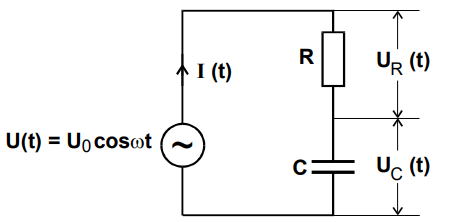
\includegraphics[height=5cm]{abbildungen/oszillatorisch.png}
    \caption{Schaltbild für den schwingenden RC-Kreis \cite{man:v353}.}
    \label{fig:schwingend}
\end{figure}